\documentclass[math,code]{amznotes}
\setcounter{tocdepth}{2}  % Only show sections in the ToC
\usepackage[utf8]{inputenc}
\usepackage{amsmath}
\usepackage{amsfonts}
\usepackage{graphicx}
\usepackage{tikz}
\usepackage{etoolbox}
\usepackage{tabularx}
\usepackage{float} % Needed for [H] placement specifier

\graphicspath{ {./images/} }
\geometry{
    a4paper,
    headheight = 1.5cm
}

\patchcmd{\chapter}{\thispagestyle{plain}}{\thispagestyle{fancy}}{}{}

\theoremstyle{remark}
\newtheorem*{claim}{Claim}
\newtheorem*{remark}{Remark}
\newtheorem{case}{Case}

\begin{document}
\fancyhead[L]{
    Engineering Calculus
}
\fancyhead[R]{
    Lecture Notes
}
\tableofcontents

\chapter{Partial Derivatives}
\section{Functions of Several Variables}
\subsection{Functions of Two variables}
\begin{dfnbox}{Functions of Two Variables}{function-of-two-variables}
    A function $\symbfit{f}$ of two variables is a rule that assigns to each ordered pair of real numbers $(x,y)$ in a set $\symbfit{D}$ a {\color{red} \textbf{unique}} real number denoted by $f(x,y)$. The set $D$ is the {\color{red} \textbf{domain}} of $f$ and its {\color{red} \textbf{range}} is the set of values that $f$ takes on, that is
    \begin{displaymath}
        \left\{ \, f(x,y) \mid (x,y) \in \symbfit{D} \, \right\}
    \end{displaymath}
\end{dfnbox}
We often write $z=f(x,y)$ to make explicit the value taken on by $\symbfit{f}$ at the general point $(x,y)$. The variables $\symbfit{x}$ and $\symbfit{y}$ are {\color{red} \textbf{independent variables}} and $\symbfit{z}$ is the {\color{red} \textbf{dependent variable}}.
\begin{notebox}
    \begin{remark}
        Compare this with the notation $y=f(x)$ for functions of a {\color{red} \textbf{single variable}}.
    \end{remark}
\end{notebox}
\subsection{Visualization}
Let's take functions of two variables as an example.
\begin{exbox}{Arrow Diagram for Functions of Two Variables}{arrow-diagram}
    A function of two variables is just a function whose domain is a subset of $R^2$ and whose range is a subset of $R$. Then, we can draw the arrow diagram like below:
    \begin{figure}[H]
    \centering
    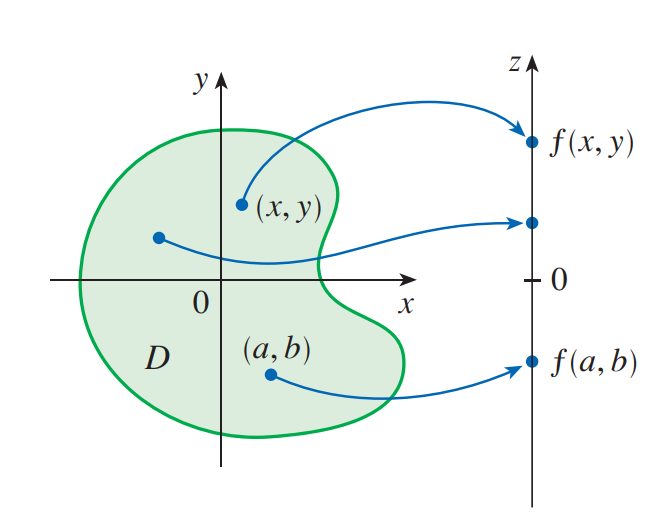
\includegraphics[width=0.35\linewidth]{images/arrow-diagram.png}
    \caption{Arrow Diagram}
    \label{fig:arrow-diagram}
    \end{figure}
\end{exbox}
\subsection{Graph}
Knowing the figure \ref{fig:arrow-diagram}, we can reform the diagram into a three dimensional coordinate system. And here comes the definition of \textbf{graph}
\begin{dfnbox}{Graph of functions of two variables}{graph-of-function-of-two-variables}
    If $\symbfit{f}$ is a function of two variables within domain $\symbfit{D}$, then the {\color{red} \textbf{graph}} of $\symbfit{f}$ is the set of all points $(x,y,z)$ in $R^3$ such that $\symbfit{z}=f(x,y)$ and $(x,y)$ is in $\symbfit{D}$.
\end{dfnbox}
\begin{notebox}
    \begin{remark}
        Usually we can think $\symbfit{z}$ and $\symbfit{f(x,y)}$ are the same.
    \end{remark}
\end{notebox}
Now, let's see an example about how the graph for a function of two variables looks like.
\begin{exbox}{Graph of functions of two variables}{graph}
    In this figure \ref{fig:graph}, the area $\symbfit{S}$ is the graph of a function of two variables.
    \begin{figure}[H]
        \centering
        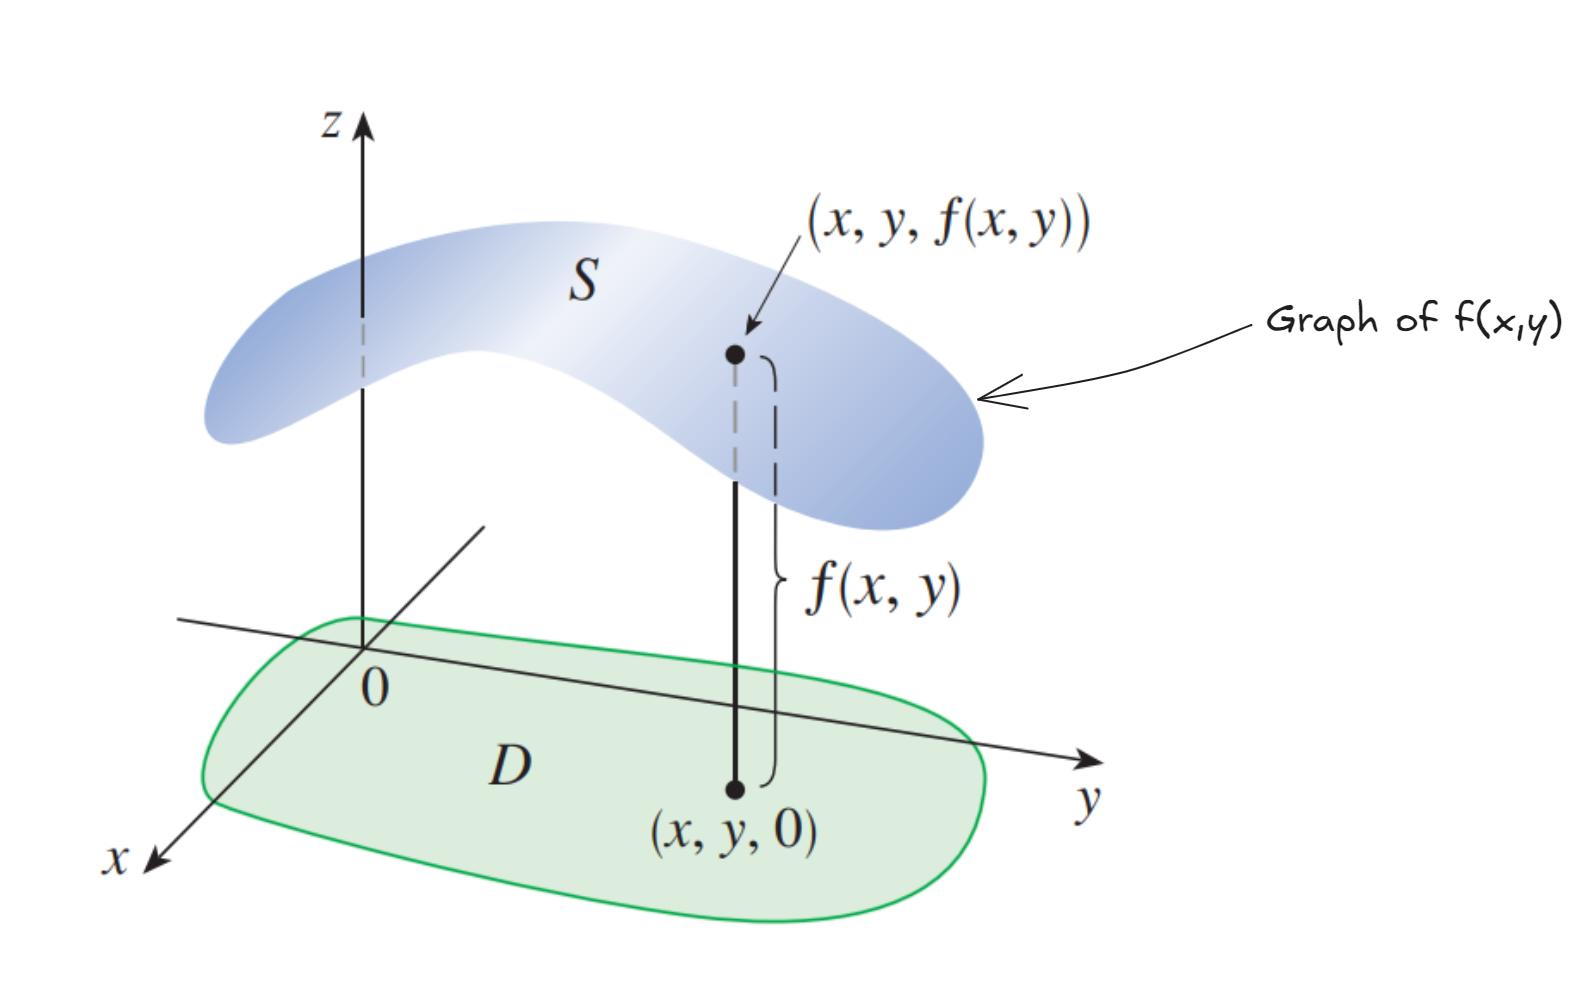
\includegraphics[width=0.5\linewidth]{images/graph.png}
        \caption{Graph}
        \label{fig:graph}
    \end{figure}
\end{exbox}
\begin{notebox}
    \begin{remark}
        In this example, the graph of the function is a \textbf{surface}. Graph is a more general concept and we can think that \textit{surface} is just one kind of \textit{graph} of a function.
    \end{remark}
\end{notebox}
\subsection{Level Curves}
\begin{dfnbox}{Level Curve}{levelcurve}
    The {\color{red} \textbf{level curves}} of a function $\symbfit{f}$ of two variables are the curves with equations $f(x,y)=\symbfit{k}$, where $\symbfit{k}$ is a constant (in the range of $\symbfit{f}$).
\end{dfnbox}
\begin{notebox}
    \begin{remark}
        From the definition of \nameref{dfn:levelcurve}, we should notice that a {\color{red} \textbf{level curve}} is the set of points in the domain of $\symbfit{f}$ at which $\symbfit{f}$ takes on a given value $\symbfit{k}$. In other words, it is a curve in {\color{red} $\symbfit{xy}$-plane} that shows where the graph of $\symbfit{f}$ has height $\symbfit{k}$ (above or below the $\symbfit{xy}$-plane).
    \end{remark}
\end{notebox}
\begin{exbox}{Find Level Curves}{findlevelcurves}
    Sketch the level curves of the function $f(x,y)=6-3x-2y$ for the values $k=-6,0,6,12$ \newline
    {\color{blue} \textbf{Solution}}: We just need to solve $6-3x-2y=k$, where $k=-6,0,6,12$. And then we will get four equations of line. We just need to plot these four lines out.
    \begin{figure}[H]
        \centering
        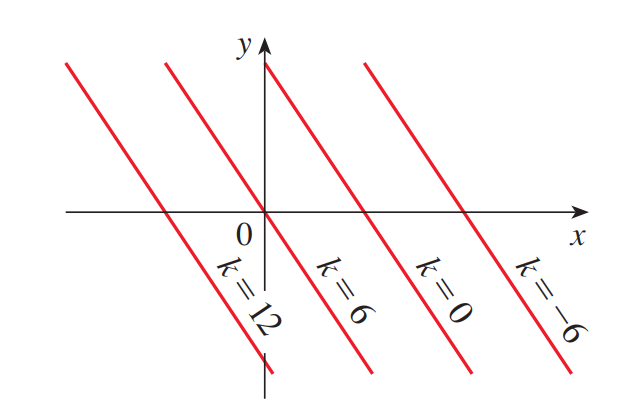
\includegraphics[width=0.5\linewidth]{images/level-curve-example.png}
        \caption{Level Curve Examples}
        \label{fig:level-curve-examples}
    \end{figure}
    In this example, we have a function of two variables and its graph should be in $R^3$, but since we need to find its level curves. To find level curves, we need to decrease the dimension by 1, so its level curves are in $R^2$.
\end{exbox}
\subsection{Contour Curves}
In the functions of two variables, we've seen that its level curves must be in $R^2$. But thinking it deeply, how does level curves come? Basically, it is the projection of \textbf{contour curves} onto the $\symbfit{xy}$-plane. So, what is the \textbf{contour plane}?
\begin{dfnbox}{Contour Curve}{contourcurve}
    For a function of two variables, denoted by $z=f(x,y)$. A horizontal plane $z=k$ may or may not intersect with the graph of $\symbfit{f}$ along a curve. If the curve exists, we say that the curve is a {\color{red} \textbf{contour curve of height $k$}}. If not, we say the contour curve doesn't exist at height $k$ for the function $\symbfit{f}$.
\end{dfnbox}
To visual it more directly, let's see the example below
\begin{exbox}{Contour Curves Example}{contour-curve-examples}
    In this figure \ref{fig:contour-curves-example}, the \textit{horizontal races} are the same as \textit{contour curves} we've discussed above.
    \begin{figure}[H]
        \centering
        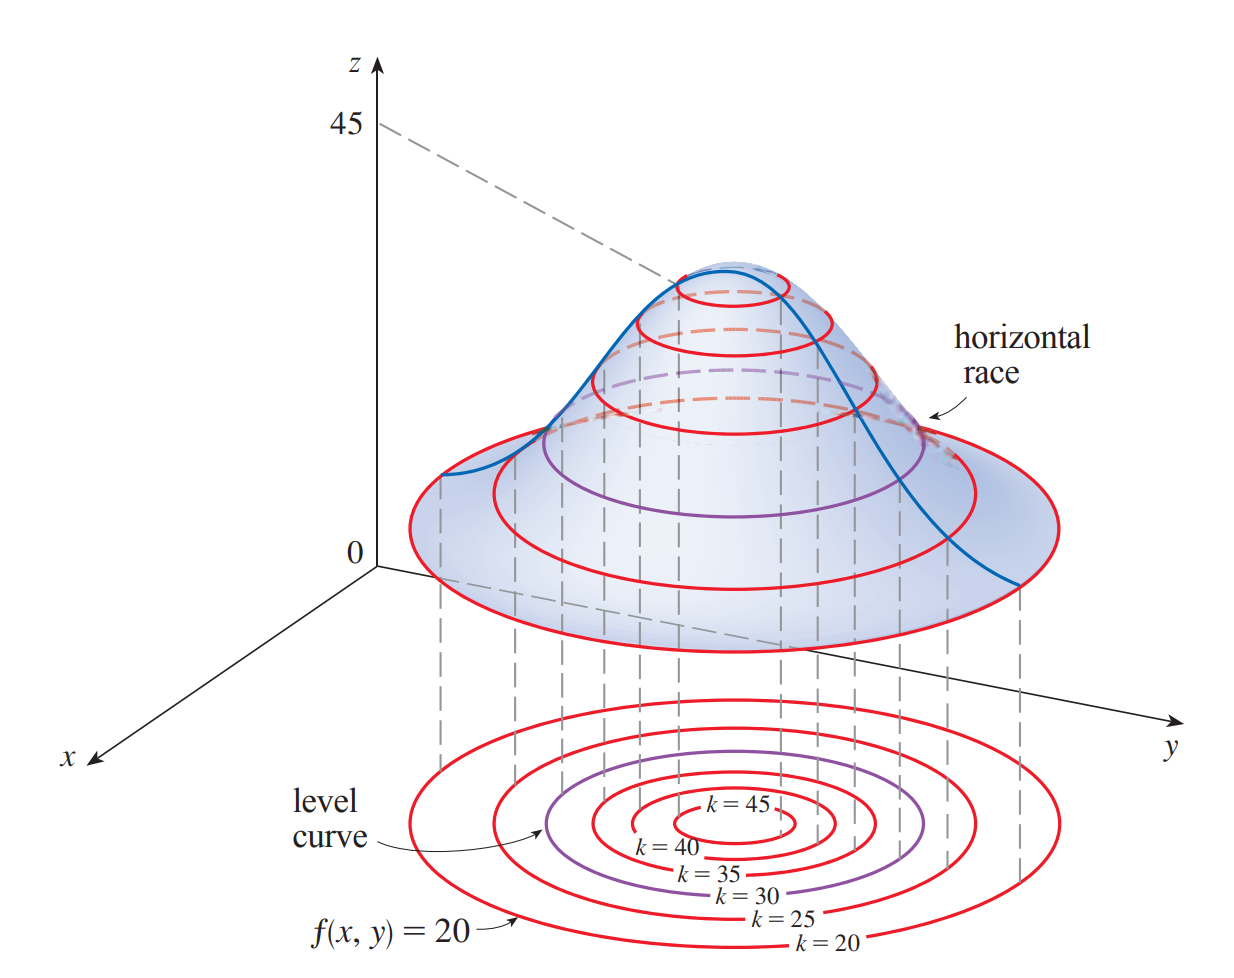
\includegraphics[width=0.5\linewidth]{images/contour-curve-example.png}
        \caption{Contour Curves Example}
        \label{fig:contour-curves-example}
    \end{figure}
\end{exbox}
\begin{notebox}
    \begin{remark}
        Sometimes, contour curves are also called \textbf{contour maps}.
    \end{remark}
\end{notebox}
\subsection{Functions of Three of more variables}
It's very difficult to visualize a function $f$ of three variables by its graph, since that would lie in $R^4$. However, we do gain some insight into $f$ by examining its {\color{red} \textbf{level surfaces}}, which are surfaces with equations $f(x,y,z)=k$, where $k$ is a constant.
\begin{exbox}{Find level surfaces}{find-level-surfaces}
    Find the level surfaces of the function
    \begin{displaymath}
        f(x,y,z)=x^2+y^2+z^2
    \end{displaymath}
    {\color{blue} \textbf{Solution}}: The level surfaces are
    \begin{displaymath}
        x^2+y^2+z^2=k, ~where~ k\geq 0
    \end{displaymath}
    These form a family of concentric spheres of the function.
\end{exbox}

\section{Limits and Continuity}
\subsection{Limits}
\begin{dfnbox}{Limits}{limits}
    Let $\symbfit{f}$ be a function of two variables whose domain $\symbfit{D}$ includes points arbitrarily close to $(a,b)$. Then we say that the {\color{red} \textbf{limits of $f(x,y)$} as $(x,y)$ approaches $(a,b)$} is $\symbfit{L}$ and we write
    \begin{displaymath}
        \lim\limits_{(x,y) \to (a,b)} f(x,y) = L
    \end{displaymath}
    if for every number $\epsilon > 0$ there is a corresponding number $\delta > 0$ such that if $(x,y) \in D$ and $0 < \sqrt{(x-a)^2+(y-b)^2} < \delta$, then $\mid f(x,y) - L \mid < \epsilon$
\end{dfnbox}
\begin{exbox}{Explanation of Limits Definition}{explanation-limits-definition}
    Basically, it says that the distance between $f(x,y)$ and $L$ can be made arbitrarily small by making the distance from $(x,y)$ to $(a,b)$ sufficiently small, but not $0$. Let's form its arrow diagram as below,
    \begin{figure}[H]
        \centering
        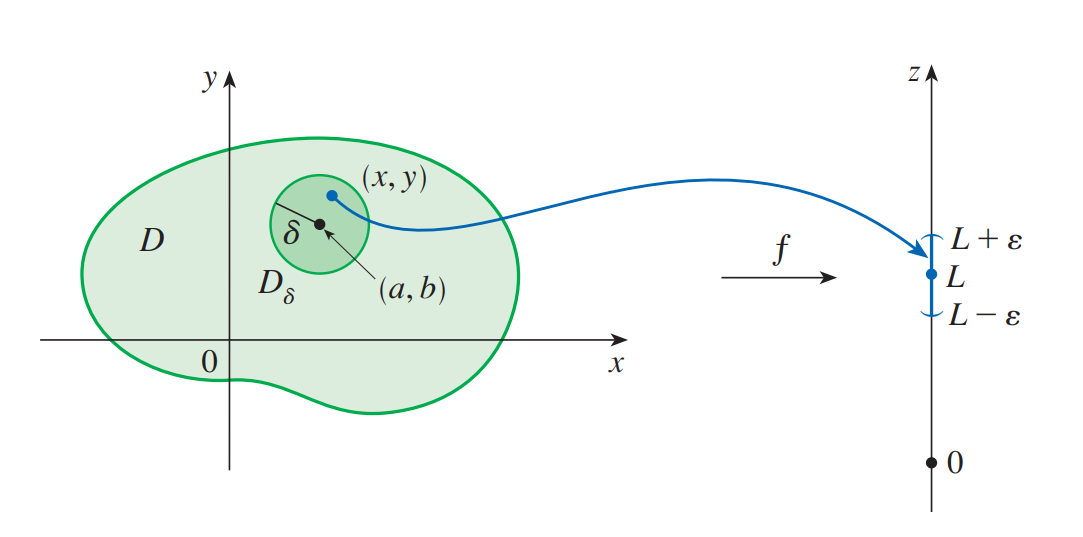
\includegraphics[width=0.5\linewidth]{images/limits-illustration.png}
        \caption{Limits Definition Explanation}
        \label{fig:limits-definition-explanation}
    \end{figure}
    From this figure \ref{fig:limits-definition-explanation}, we can see that if any small interval $(L - \epsilon, L + \epsilon)$ is given around $L$, then we can find a disk $D_\delta$ with center $(a,b)$ and radius $\delta > 0$ such that $\symbfit{f}$ maps all the points in $D_\delta$ \text{[except possibly $(a,b)$]} into the interval $(L - \epsilon, L + \epsilon)$
\end{exbox}
\subsubsection{Show that a limit doesn't exist}
Since in the definition of \nameref{dfn:limits}, it refers only to the \textbf{distance} between $(x,y)$ and $(a,b)$. It does not refer to the \textbf{direction} of approach. Therefore, if the limit exists, then $f(x,y)$ must approach the same limit \textbf{no matter how} $(x,y)$ approaches $(a,b)$. Thus, one way to show that $\lim\limits_{(x,y) \to (a,b)} f(x,y)$ does not exist is to find {\color{red} \textbf{different paths}} of approach along which the function has different limits.
\begin{notebox}
    \begin{claim}
        If $f(x,y) \to L_1$ as $(x,y) \to (a,b)$ along a path $C_1$ and $f(x,y) \to L_2$ as $(x,y) \to (a,b)$ along a path $C_2$, where $L_1 \neq L_2$, then $\lim\limits_{(x,y) \to (a,b)} f(x,y)$ does not exist.
    \end{claim}
\end{notebox}
\begin{exbox}{Limit does not exist}{limits-dne}
    Show that $\lim\limits_{(x,y) \to (0,0)} \frac{x^2-y^2}{x^2+y^2}$ does not exist \newline
    {\color{blue} \textbf{Solution}}:
    \begin{enumerate}
        \item Let's approach $(0,0)$ along the $x$-axis. On this path $y=0$, the function becomes $f(x,0)=\frac{x^2}{x^2}=1, \forall x \neq 0$ and thus
        \begin{displaymath}
            f(x,y) \to 1 \text{ as } (x,y) \to (0,0) \text{ along the }x \text{-axis.}
        \end{displaymath}
        \item We now approach along the $y$-axis by putting $x=0$. Then $f(0,y)=\frac{-y^2}{y^2}=-1, \forall y \neq 0$, so
        \begin{displaymath}
            (x,y) \to -1 \text{ as } (x,y) \to (0,0) \text{ along the }y \text{-axis.}
        \end{displaymath}
        So, DNE!
    \end{enumerate}
\end{exbox}
\subsubsection{Properties of Limits}
Before we talk about the properties, let's give two definitions about the \textbf{polynomial function} and the \textbf{rational function}.
\begin{dfnbox}{Polynomial Function}{polynomial-function}
    A {\color{red} \textbf{polynomial function}} of two variables (or polynomial, for short) is a sum of terms of the form ($x^my^n$, where $\symbfit{c}$ is a constant and $\symbfit{m}$ and $\symbfit{n}$ are \textbf{non-negative integers}. For example,
    \begin{displaymath}
        p(x,y)=x^4+5x^3y^2+6xy^4-7y+6
    \end{displaymath}
\end{dfnbox}
\begin{dfnbox}{Rational Function}{rational-function}
    A {\color{red} \textbf{rational function}} is a ratio of two \nameref{dfn:polynomial-function}s. For example,
    \begin{displaymath}
        q(x,y)=\frac{2xy+1}{x^2+y^2}
    \end{displaymath}
\end{dfnbox}
Now, we state that
\begin{notebox}
    \begin{claim}
        To find the limit of any polynomial function, we can use \textbf{direct substitution}. For example,
        \begin{displaymath}
            \lim\limits_{(x,y) \to (a,b)} p(x,y) = p(a,,b)
        \end{displaymath}
    \end{claim}
\end{notebox}
and,
\begin{notebox}
    \begin{claim}
        To find the limit of any rational function, we have
        \begin{displaymath}
            \lim\limits_{(x,y) \to (a,b)} q(x,y) = \lim\limits_{(x,y) \to (a,b)} \frac{p(x,y)}{r(x,y)} = \frac{p(a,b)}{r(a,b)}=q(a,b)
        \end{displaymath}
        provided that $(a,b)$ is in the domain of $q$. If not, we need to use the definition about limits does not exist.
    \end{claim}
\end{notebox}
\subsection{Continuity}
\begin{dfnbox}{Continuity}{continuity}
    A function $\symbfit{f}$ of two variables is called {\color{red} \textbf{continuous}} at $(a,b)$ if
    \begin{displaymath}
        \lim\limits_{(x,y) \to (a,b)} f(x,y) = f(a,b)
    \end{displaymath}
    We say that $\symbfit{f}$ is {\color{red} \textbf{continuous}} on $\symbfit{D}$ if $\symbfit{f}$ is continuous at every point $(a,b)$ in $\symbfit{D}$.
\end{dfnbox}
\end{document}